% Options for packages loaded elsewhere
\PassOptionsToPackage{unicode}{hyperref}
\PassOptionsToPackage{hyphens}{url}
\documentclass[
  11pt,
]{article}
\usepackage{xcolor}
\usepackage[margin=1in]{geometry}
\usepackage{amsmath,amssymb}
\setcounter{secnumdepth}{5}
\usepackage{iftex}
\ifPDFTeX
  \usepackage[T1]{fontenc}
  \usepackage[utf8]{inputenc}
  \usepackage{textcomp} % provide euro and other symbols
\else % if luatex or xetex
  \usepackage{unicode-math} % this also loads fontspec
  \defaultfontfeatures{Scale=MatchLowercase}
  \defaultfontfeatures[\rmfamily]{Ligatures=TeX,Scale=1}
\fi
\usepackage{lmodern}
\ifPDFTeX\else
  % xetex/luatex font selection
\fi
% Use upquote if available, for straight quotes in verbatim environments
\IfFileExists{upquote.sty}{\usepackage{upquote}}{}
\IfFileExists{microtype.sty}{% use microtype if available
  \usepackage[]{microtype}
  \UseMicrotypeSet[protrusion]{basicmath} % disable protrusion for tt fonts
}{}
\makeatletter
\@ifundefined{KOMAClassName}{% if non-KOMA class
  \IfFileExists{parskip.sty}{%
    \usepackage{parskip}
  }{% else
    \setlength{\parindent}{0pt}
    \setlength{\parskip}{6pt plus 2pt minus 1pt}}
}{% if KOMA class
  \KOMAoptions{parskip=half}}
\makeatother
\usepackage{color}
\usepackage{fancyvrb}
\newcommand{\VerbBar}{|}
\newcommand{\VERB}{\Verb[commandchars=\\\{\}]}
\DefineVerbatimEnvironment{Highlighting}{Verbatim}{commandchars=\\\{\}}
% Add ',fontsize=\small' for more characters per line
\usepackage{framed}
\definecolor{shadecolor}{RGB}{248,248,248}
\newenvironment{Shaded}{\begin{snugshade}}{\end{snugshade}}
\newcommand{\AlertTok}[1]{\textcolor[rgb]{0.94,0.16,0.16}{#1}}
\newcommand{\AnnotationTok}[1]{\textcolor[rgb]{0.56,0.35,0.01}{\textbf{\textit{#1}}}}
\newcommand{\AttributeTok}[1]{\textcolor[rgb]{0.13,0.29,0.53}{#1}}
\newcommand{\BaseNTok}[1]{\textcolor[rgb]{0.00,0.00,0.81}{#1}}
\newcommand{\BuiltInTok}[1]{#1}
\newcommand{\CharTok}[1]{\textcolor[rgb]{0.31,0.60,0.02}{#1}}
\newcommand{\CommentTok}[1]{\textcolor[rgb]{0.56,0.35,0.01}{\textit{#1}}}
\newcommand{\CommentVarTok}[1]{\textcolor[rgb]{0.56,0.35,0.01}{\textbf{\textit{#1}}}}
\newcommand{\ConstantTok}[1]{\textcolor[rgb]{0.56,0.35,0.01}{#1}}
\newcommand{\ControlFlowTok}[1]{\textcolor[rgb]{0.13,0.29,0.53}{\textbf{#1}}}
\newcommand{\DataTypeTok}[1]{\textcolor[rgb]{0.13,0.29,0.53}{#1}}
\newcommand{\DecValTok}[1]{\textcolor[rgb]{0.00,0.00,0.81}{#1}}
\newcommand{\DocumentationTok}[1]{\textcolor[rgb]{0.56,0.35,0.01}{\textbf{\textit{#1}}}}
\newcommand{\ErrorTok}[1]{\textcolor[rgb]{0.64,0.00,0.00}{\textbf{#1}}}
\newcommand{\ExtensionTok}[1]{#1}
\newcommand{\FloatTok}[1]{\textcolor[rgb]{0.00,0.00,0.81}{#1}}
\newcommand{\FunctionTok}[1]{\textcolor[rgb]{0.13,0.29,0.53}{\textbf{#1}}}
\newcommand{\ImportTok}[1]{#1}
\newcommand{\InformationTok}[1]{\textcolor[rgb]{0.56,0.35,0.01}{\textbf{\textit{#1}}}}
\newcommand{\KeywordTok}[1]{\textcolor[rgb]{0.13,0.29,0.53}{\textbf{#1}}}
\newcommand{\NormalTok}[1]{#1}
\newcommand{\OperatorTok}[1]{\textcolor[rgb]{0.81,0.36,0.00}{\textbf{#1}}}
\newcommand{\OtherTok}[1]{\textcolor[rgb]{0.56,0.35,0.01}{#1}}
\newcommand{\PreprocessorTok}[1]{\textcolor[rgb]{0.56,0.35,0.01}{\textit{#1}}}
\newcommand{\RegionMarkerTok}[1]{#1}
\newcommand{\SpecialCharTok}[1]{\textcolor[rgb]{0.81,0.36,0.00}{\textbf{#1}}}
\newcommand{\SpecialStringTok}[1]{\textcolor[rgb]{0.31,0.60,0.02}{#1}}
\newcommand{\StringTok}[1]{\textcolor[rgb]{0.31,0.60,0.02}{#1}}
\newcommand{\VariableTok}[1]{\textcolor[rgb]{0.00,0.00,0.00}{#1}}
\newcommand{\VerbatimStringTok}[1]{\textcolor[rgb]{0.31,0.60,0.02}{#1}}
\newcommand{\WarningTok}[1]{\textcolor[rgb]{0.56,0.35,0.01}{\textbf{\textit{#1}}}}
\usepackage{graphicx}
\makeatletter
\newsavebox\pandoc@box
\newcommand*\pandocbounded[1]{% scales image to fit in text height/width
  \sbox\pandoc@box{#1}%
  \Gscale@div\@tempa{\textheight}{\dimexpr\ht\pandoc@box+\dp\pandoc@box\relax}%
  \Gscale@div\@tempb{\linewidth}{\wd\pandoc@box}%
  \ifdim\@tempb\p@<\@tempa\p@\let\@tempa\@tempb\fi% select the smaller of both
  \ifdim\@tempa\p@<\p@\scalebox{\@tempa}{\usebox\pandoc@box}%
  \else\usebox{\pandoc@box}%
  \fi%
}
% Set default figure placement to htbp
\def\fps@figure{htbp}
\makeatother
% definitions for citeproc citations
\NewDocumentCommand\citeproctext{}{}
\NewDocumentCommand\citeproc{mm}{%
  \begingroup\def\citeproctext{#2}\cite{#1}\endgroup}
\makeatletter
 % allow citations to break across lines
 \let\@cite@ofmt\@firstofone
 % avoid brackets around text for \cite:
 \def\@biblabel#1{}
 \def\@cite#1#2{{#1\if@tempswa , #2\fi}}
\makeatother
\newlength{\cslhangindent}
\setlength{\cslhangindent}{1.5em}
\newlength{\csllabelwidth}
\setlength{\csllabelwidth}{3em}
\newenvironment{CSLReferences}[2] % #1 hanging-indent, #2 entry-spacing
 {\begin{list}{}{%
  \setlength{\itemindent}{0pt}
  \setlength{\leftmargin}{0pt}
  \setlength{\parsep}{0pt}
  % turn on hanging indent if param 1 is 1
  \ifodd #1
   \setlength{\leftmargin}{\cslhangindent}
   \setlength{\itemindent}{-1\cslhangindent}
  \fi
  % set entry spacing
  \setlength{\itemsep}{#2\baselineskip}}}
 {\end{list}}
\usepackage{calc}
\newcommand{\CSLBlock}[1]{\hfill\break\parbox[t]{\linewidth}{\strut\ignorespaces#1\strut}}
\newcommand{\CSLLeftMargin}[1]{\parbox[t]{\csllabelwidth}{\strut#1\strut}}
\newcommand{\CSLRightInline}[1]{\parbox[t]{\linewidth - \csllabelwidth}{\strut#1\strut}}
\newcommand{\CSLIndent}[1]{\hspace{\cslhangindent}#1}
\setlength{\emergencystretch}{3em} % prevent overfull lines
\providecommand{\tightlist}{%
  \setlength{\itemsep}{0pt}\setlength{\parskip}{0pt}}
\usepackage{float}
\usepackage{bookmark}
\IfFileExists{xurl.sty}{\usepackage{xurl}}{} % add URL line breaks if available
\urlstyle{same}
\hypersetup{
  pdftitle={Task 3},
  pdfauthor={Simon Safron {[}Mn: 11923407{]}, Alexander Veith {[}Mn: 12122739{]}, Miriam Überbacher {[}Mn:01627576{]}},
  hidelinks,
  pdfcreator={LaTeX via pandoc}}

\title{Task 3}
\author{Simon Safron {[}Mn: 11923407{]}, Alexander Veith {[}Mn:
12122739{]}, Miriam Überbacher {[}Mn:01627576{]}}
\date{2025-12-06}

\begin{document}
\maketitle

{
\setcounter{tocdepth}{2}
\tableofcontents
}
\section{Introduction}\label{introduction}

{[}Add introduction text here{]}

\section{Raw Reads and Mapping Quality
Control}\label{raw-reads-and-mapping-quality-control}

\subsection{FastQC Analysis}\label{fastqc-analysis}

\subsubsection{a) Sequencing Depth per
Sample}\label{a-sequencing-depth-per-sample}

\begin{figure}[H]

{\centering 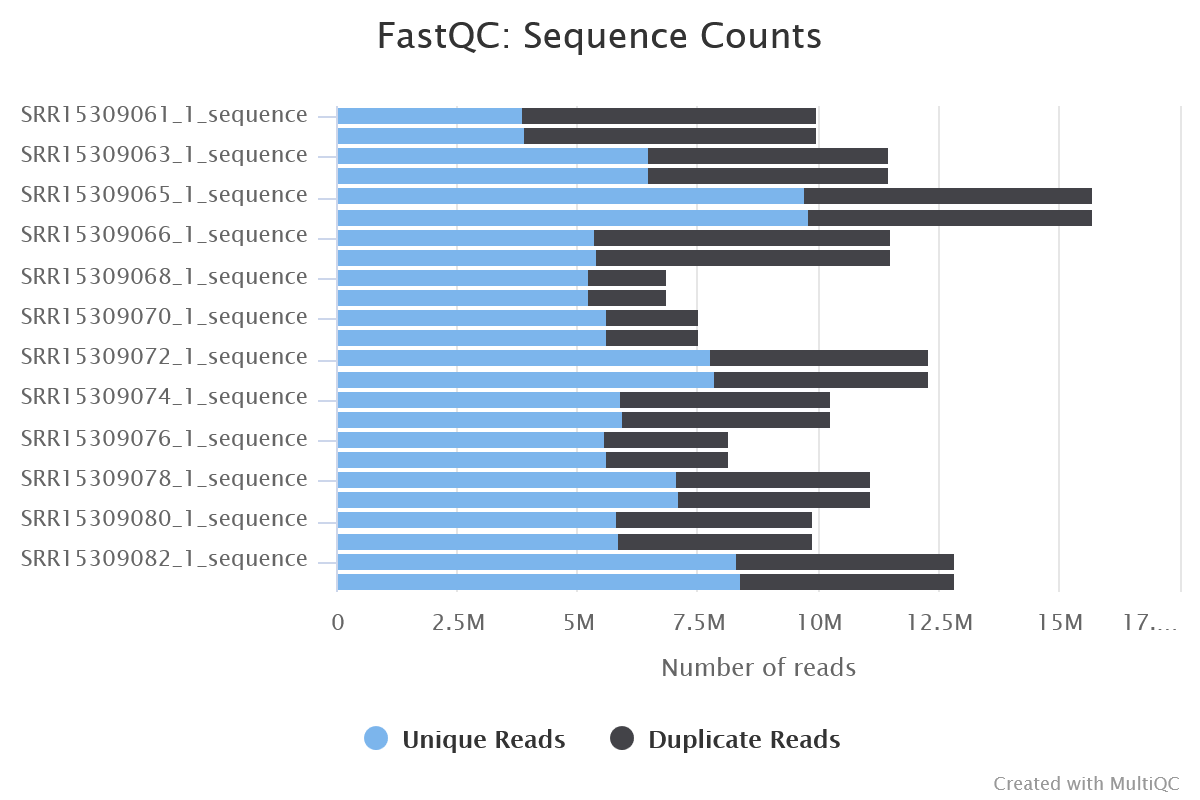
\includegraphics[width=0.85\linewidth]{fastqc_sequence_counts_plot} 

}

\caption{Barplot of the number of read pairs per sample as reported by FastQC.}\label{fig:unnamed-chunk-1}
\end{figure}

According to FastQC (Figure 1), the minimum number of read pairs per
sample is approximately 6.8 million, while the maximum is approximately
15.7 million.

\subsubsection{b) Most Overrepresented
Sequence}\label{b-most-overrepresented-sequence}

According to the MultiQC report, the most overrepresented sequence
detected by FastQC was:

\begin{verbatim}
AAAAAAAAAAAAAAAAAAAAAAAAAAAAAAAAAAAAAAAAAAAAAAAAAAAA
\end{verbatim}

\subsubsection{c) Potential Source of Homopolymer
Sequences}\label{c-potential-source-of-homopolymer-sequences}

This homopolymer sequence likely originates from \textbf{A-tailed
adapter dimers} and \textbf{PCR slippage products} that outcompete
genuine RNA fragments in the library construction process.

\subsection{HTSeq-count Assignment}\label{htseq-count-assignment}

\subsubsection{d) Read Pair Counts per
Sample}\label{d-read-pair-counts-per-sample}

\begin{figure}[H]

{\centering 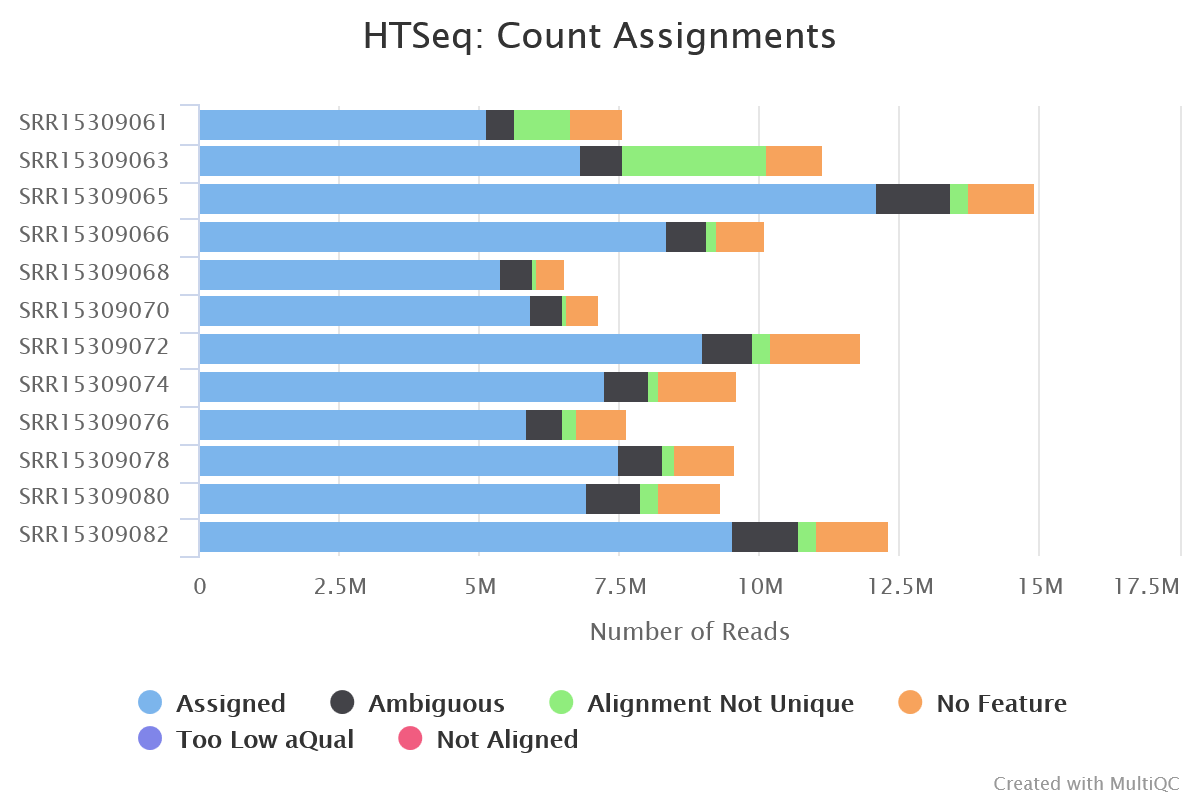
\includegraphics[width=0.85\linewidth]{htseq_assignment_plot} 

}

\caption{Barplot of the number of read pairs per sample as reported by HTSeq-count.}\label{fig:unnamed-chunk-2}
\end{figure}

According to HTSeq-count (Figure 2), the minimum number of read pairs
per sample is approximately 5.9 million, while the maximum is
approximately 14.8 million.

\subsubsection{e) Percentage of Uniquely Assigned
Reads}\label{e-percentage-of-uniquely-assigned-reads}

\begin{figure}[H]

{\centering 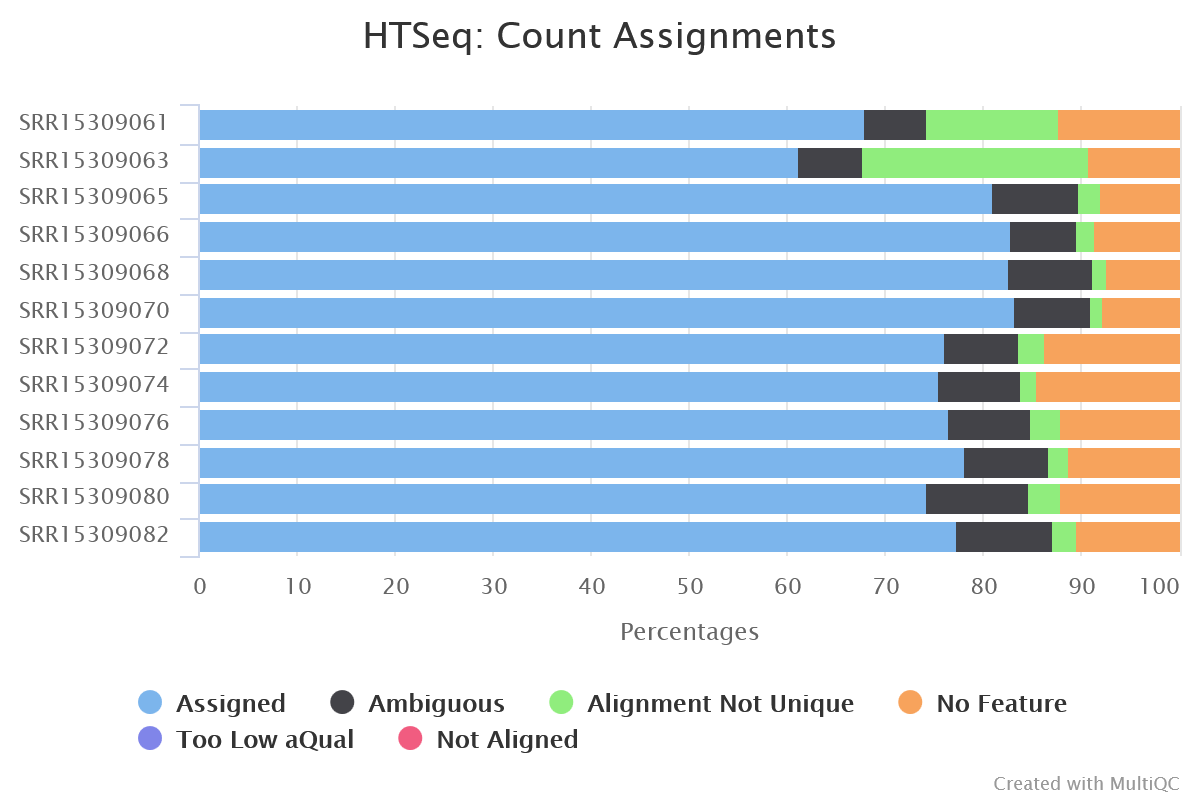
\includegraphics[width=0.85\linewidth]{htseq_assignment_plot_percentages} 

}

\caption{HTSeq assignment plot showing percentage of reads uniquely assigned to genes.}\label{fig:unnamed-chunk-3}
\end{figure}

As shown in Figure 3, the minimum percentage of reads uniquely assigned
to genes is 61.3\%, while the maximum is approximately 83.3\%.

\newpage

\section{Dataset Description}\label{dataset-description}

\subsection{Sample Information}\label{sample-information}

\subsubsection{a) Strain and Genotype
Identification}\label{a-strain-and-genotype-identification}

The \textbf{genotype} column defines the base strain (wild type vs.~TGT
mutant), while the \textbf{strain} column indicates the \emph{E. coli}
strain used.

\textbf{Identified error:} The strain column appears to suggest a
different strain for each experiment. However, the methods section of
the paper specifies that only ``Escherichia coli K-12 MG1655'' was used
as the WT strain.

\subsubsection{b) Nickel Treatment
Column}\label{b-nickel-treatment-column}

The \textbf{treatment} column defines whether nickel was added to the
media.

\subsubsection{c) SRA Study Information}\label{c-sra-study-information}

The following metadata was retrieved from the SRA Study page:

\begin{itemize}
\tightlist
\item
  \textbf{Sequencing platform:} Illumina HiSeq 2500
\item
  \textbf{Library layout:} PAIRED
\item
  \textbf{Data release date:} 2022-05-16
\end{itemize}

\subsection{Raw Count Data}\label{raw-count-data}

\section{Data Preprocessing}\label{data-preprocessing}

\subsection{Filtering Analysis}\label{filtering-analysis}

\subsubsection{a) Original Gene Count}\label{a-original-gene-count}

\begin{Shaded}
\begin{Highlighting}[]
\FunctionTok{dim}\NormalTok{(rawCounts)}
\CommentTok{\#[1] 4295   12}
\end{Highlighting}
\end{Shaded}

Originally, count data were retrieved for \textbf{4,295 genes}.

\subsubsection{b) Gene Count After
Filtering}\label{b-gene-count-after-filtering}

\begin{Shaded}
\begin{Highlighting}[]
\FunctionTok{dim}\NormalTok{(rawCounts[}\FunctionTok{rowSums}\NormalTok{(rawCounts) }\SpecialCharTok{\textgreater{}} \DecValTok{10}\NormalTok{, ])}
\CommentTok{\#[1] 4221   12}
\end{Highlighting}
\end{Shaded}

After applying the filter (rowSums \textgreater{} 10), \textbf{4,221
genes} remain.

\newpage

\section{Differential Gene Expression (DGE)
Analysis}\label{differential-gene-expression-dge-analysis}

\subsection{Extracting and Interpreting
Results}\label{extracting-and-interpreting-results}

\subsubsection{a) Differentially Expressed Genes: WT Nickel vs.~WT No
Treatment}\label{a-differentially-expressed-genes-wt-nickel-vs.-wt-no-treatment}

\begin{Shaded}
\begin{Highlighting}[]
\NormalTok{DESeq2Results\_WT\_nickel }\OtherTok{\textless{}{-}} \FunctionTok{results}\NormalTok{(}
\NormalTok{  DESeq2Data, }
  \AttributeTok{contrast =} \FunctionTok{c}\NormalTok{(}\StringTok{"group"}\NormalTok{, }\StringTok{"WT.Nickel"}\NormalTok{, }\StringTok{"WT.none"}\NormalTok{)}
\NormalTok{)}

\FunctionTok{summary}\NormalTok{(DESeq2Results\_WT\_nickel)}
\end{Highlighting}
\end{Shaded}

In the nickel-treated WT strain compared to untreated WT strain (at
p-value \textless{} 0.1), \textbf{1,069 genes are significantly
up-regulated} and \textbf{1,063 genes are significantly down-regulated}.

\subsubsection{b) Default Significance
Cutoff}\label{b-default-significance-cutoff}

The standard cutoff for adjusted p-value is \textbf{α = 0.1 (10\%)}.

\subsubsection{c) Total Significantly Differentially Expressed Genes:
TGT Nickel vs.~TGT No
Treatment}\label{c-total-significantly-differentially-expressed-genes-tgt-nickel-vs.-tgt-no-treatment}

\begin{Shaded}
\begin{Highlighting}[]
\NormalTok{DESeq2Results\_TGT\_nickel }\OtherTok{\textless{}{-}} \FunctionTok{results}\NormalTok{(}
\NormalTok{  DESeq2Data, }
  \AttributeTok{contrast =} \FunctionTok{c}\NormalTok{(}\StringTok{"group"}\NormalTok{, }\StringTok{"TGT.Nickel"}\NormalTok{, }\StringTok{"TGT.none"}\NormalTok{),}
  \AttributeTok{alpha =} \FloatTok{0.1}
\NormalTok{)}

\FunctionTok{summary}\NormalTok{(DESeq2Results\_TGT\_nickel)}
\end{Highlighting}
\end{Shaded}

The total number of significantly differentially expressed genes is
\textbf{1,863} (986 up-regulated + 877 down-regulated).

\subsection{Effect of Significance
Level}\label{effect-of-significance-level}

\subsubsection{d) Genotype Comparison at α =
0.05}\label{d-genotype-comparison-at-ux3b1-0.05}

\begin{Shaded}
\begin{Highlighting}[]
\NormalTok{DESeq2Results\_genotype }\OtherTok{\textless{}{-}} \FunctionTok{results}\NormalTok{(}
\NormalTok{  DESeq2Data, }
  \AttributeTok{contrast =} \FunctionTok{c}\NormalTok{(}\StringTok{"group"}\NormalTok{, }\StringTok{"TGT.none"}\NormalTok{, }\StringTok{"WT.none"}\NormalTok{),}
  \AttributeTok{alpha =} \FloatTok{0.05}
\NormalTok{)}

\FunctionTok{summary}\NormalTok{(DESeq2Results\_genotype)}
\end{Highlighting}
\end{Shaded}

At a significance level of α = 0.05, there are \textbf{462 significantly
differentially expressed genes} (187 up-regulated + 275 down-regulated)
when comparing TGT mutant to WT under standard conditions.

\subsubsection{e) TGT Mutant Nickel Treatment Effect at α =
0.05}\label{e-tgt-mutant-nickel-treatment-effect-at-ux3b1-0.05}

\begin{Shaded}
\begin{Highlighting}[]
\NormalTok{DESeq2Results\_TGT\_nickel }\OtherTok{\textless{}{-}} \FunctionTok{results}\NormalTok{(}
\NormalTok{  DESeq2Data, }
  \AttributeTok{contrast =} \FunctionTok{c}\NormalTok{(}\StringTok{"group"}\NormalTok{, }\StringTok{"TGT.Nickel"}\NormalTok{, }\StringTok{"TGT.none"}\NormalTok{),}
  \AttributeTok{alpha =} \FloatTok{0.05}
\NormalTok{)}

\FunctionTok{summary}\NormalTok{(DESeq2Results\_TGT\_nickel)}
\end{Highlighting}
\end{Shaded}

At a significance level of α = 0.05, there are \textbf{1,578
significantly differentially expressed genes} (826 up-regulated + 752
down-regulated) in the TGT mutant strain when comparing nickel-treated
to untreated conditions.

\newpage

\section{Data Visualization and Quality
Control}\label{data-visualization-and-quality-control}

\subsection{Experimental Quality Control: Sample Clustering
(PCA)}\label{experimental-quality-control-sample-clustering-pca}

\begin{figure}[H]

{\centering 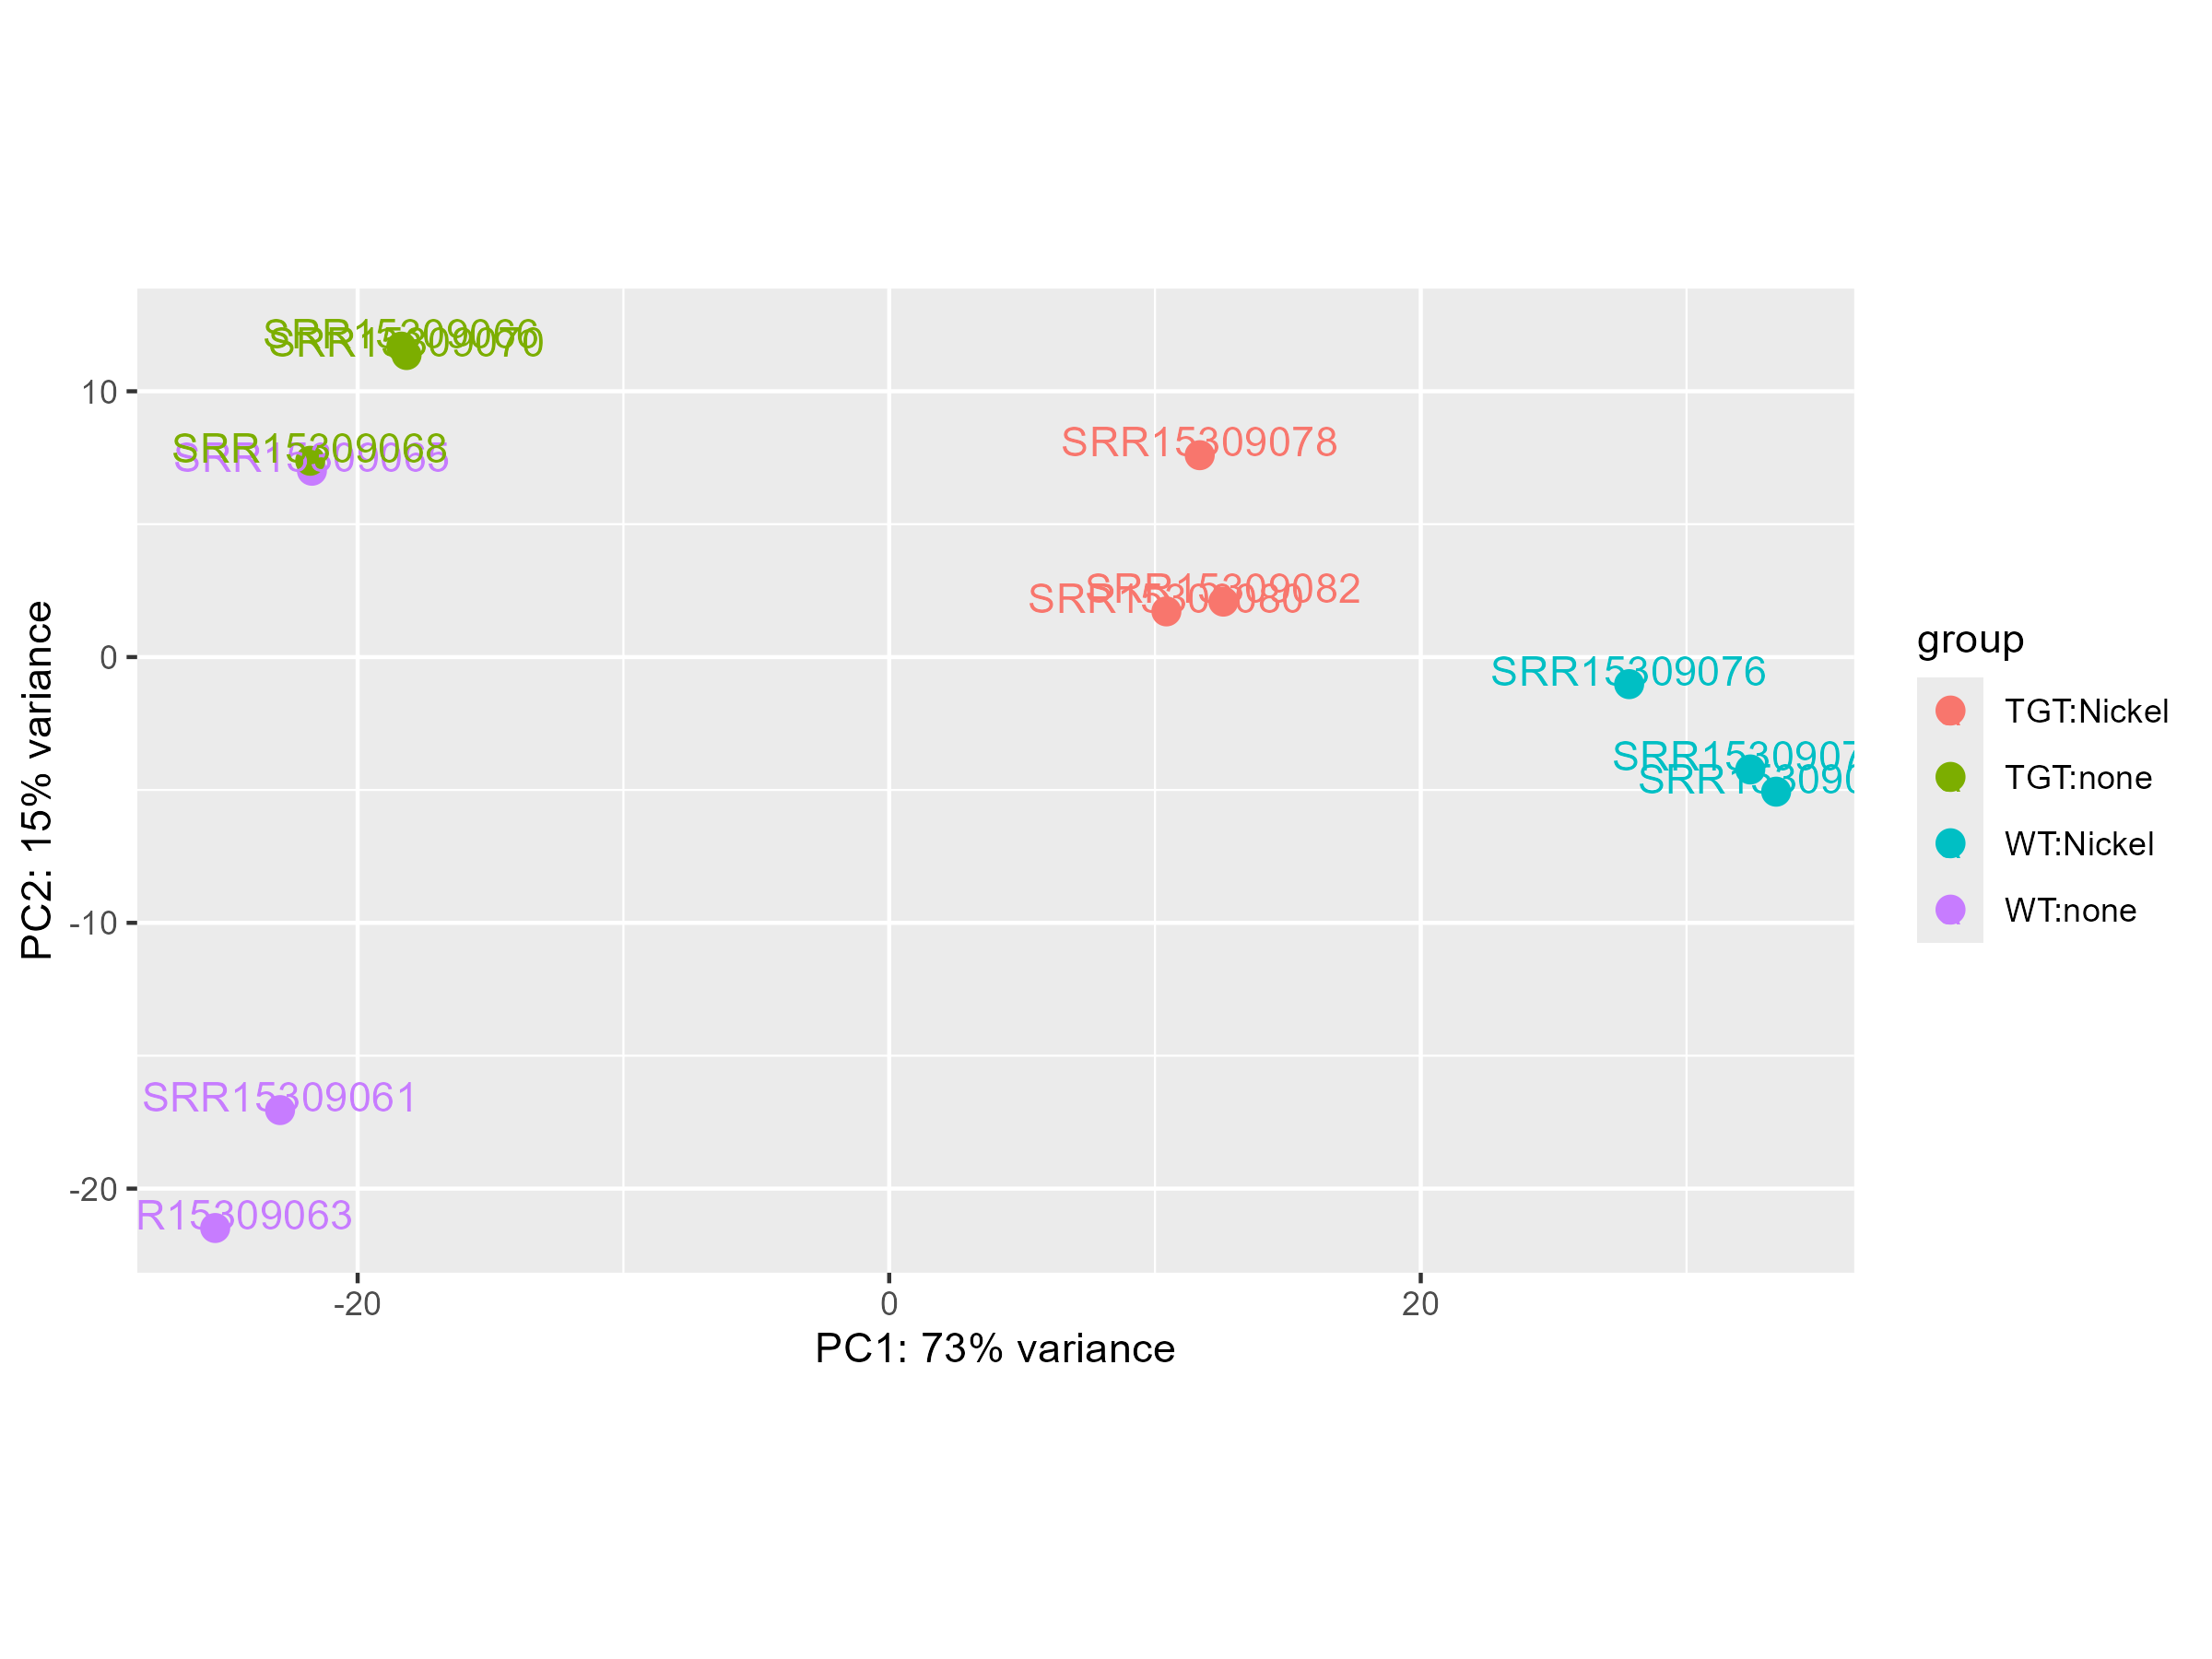
\includegraphics[width=0.85\linewidth]{PCAplot} 

}

\caption{Principal Component Analysis (PCA) plot showing clustering of samples.}\label{fig:unnamed-chunk-10}
\end{figure}

\subsubsection{a) Replicate Group
Behavior}\label{a-replicate-group-behavior}

The samples cluster as expected. Individual experimental groups are
clearly separated from each other. Notably, there is substantial
separation between untreated and nickel-treated samples for both WT and
TGT strains, which is consistent with the strong transcriptomic response
to nickel treatment.

\subsubsection{b) Outlier
Identification}\label{b-outlier-identification}

The WT untreated (WT.none) samples do not cluster perfectly together.
Specifically, one WT.none replicate clusters closer to the TGT.none
group, suggesting it may be an outlier and warrants further
investigation.

\subsection{Single Gene Expression: tgt Gene
Counts}\label{single-gene-expression-tgt-gene-counts}

\begin{figure}[H]

{\centering 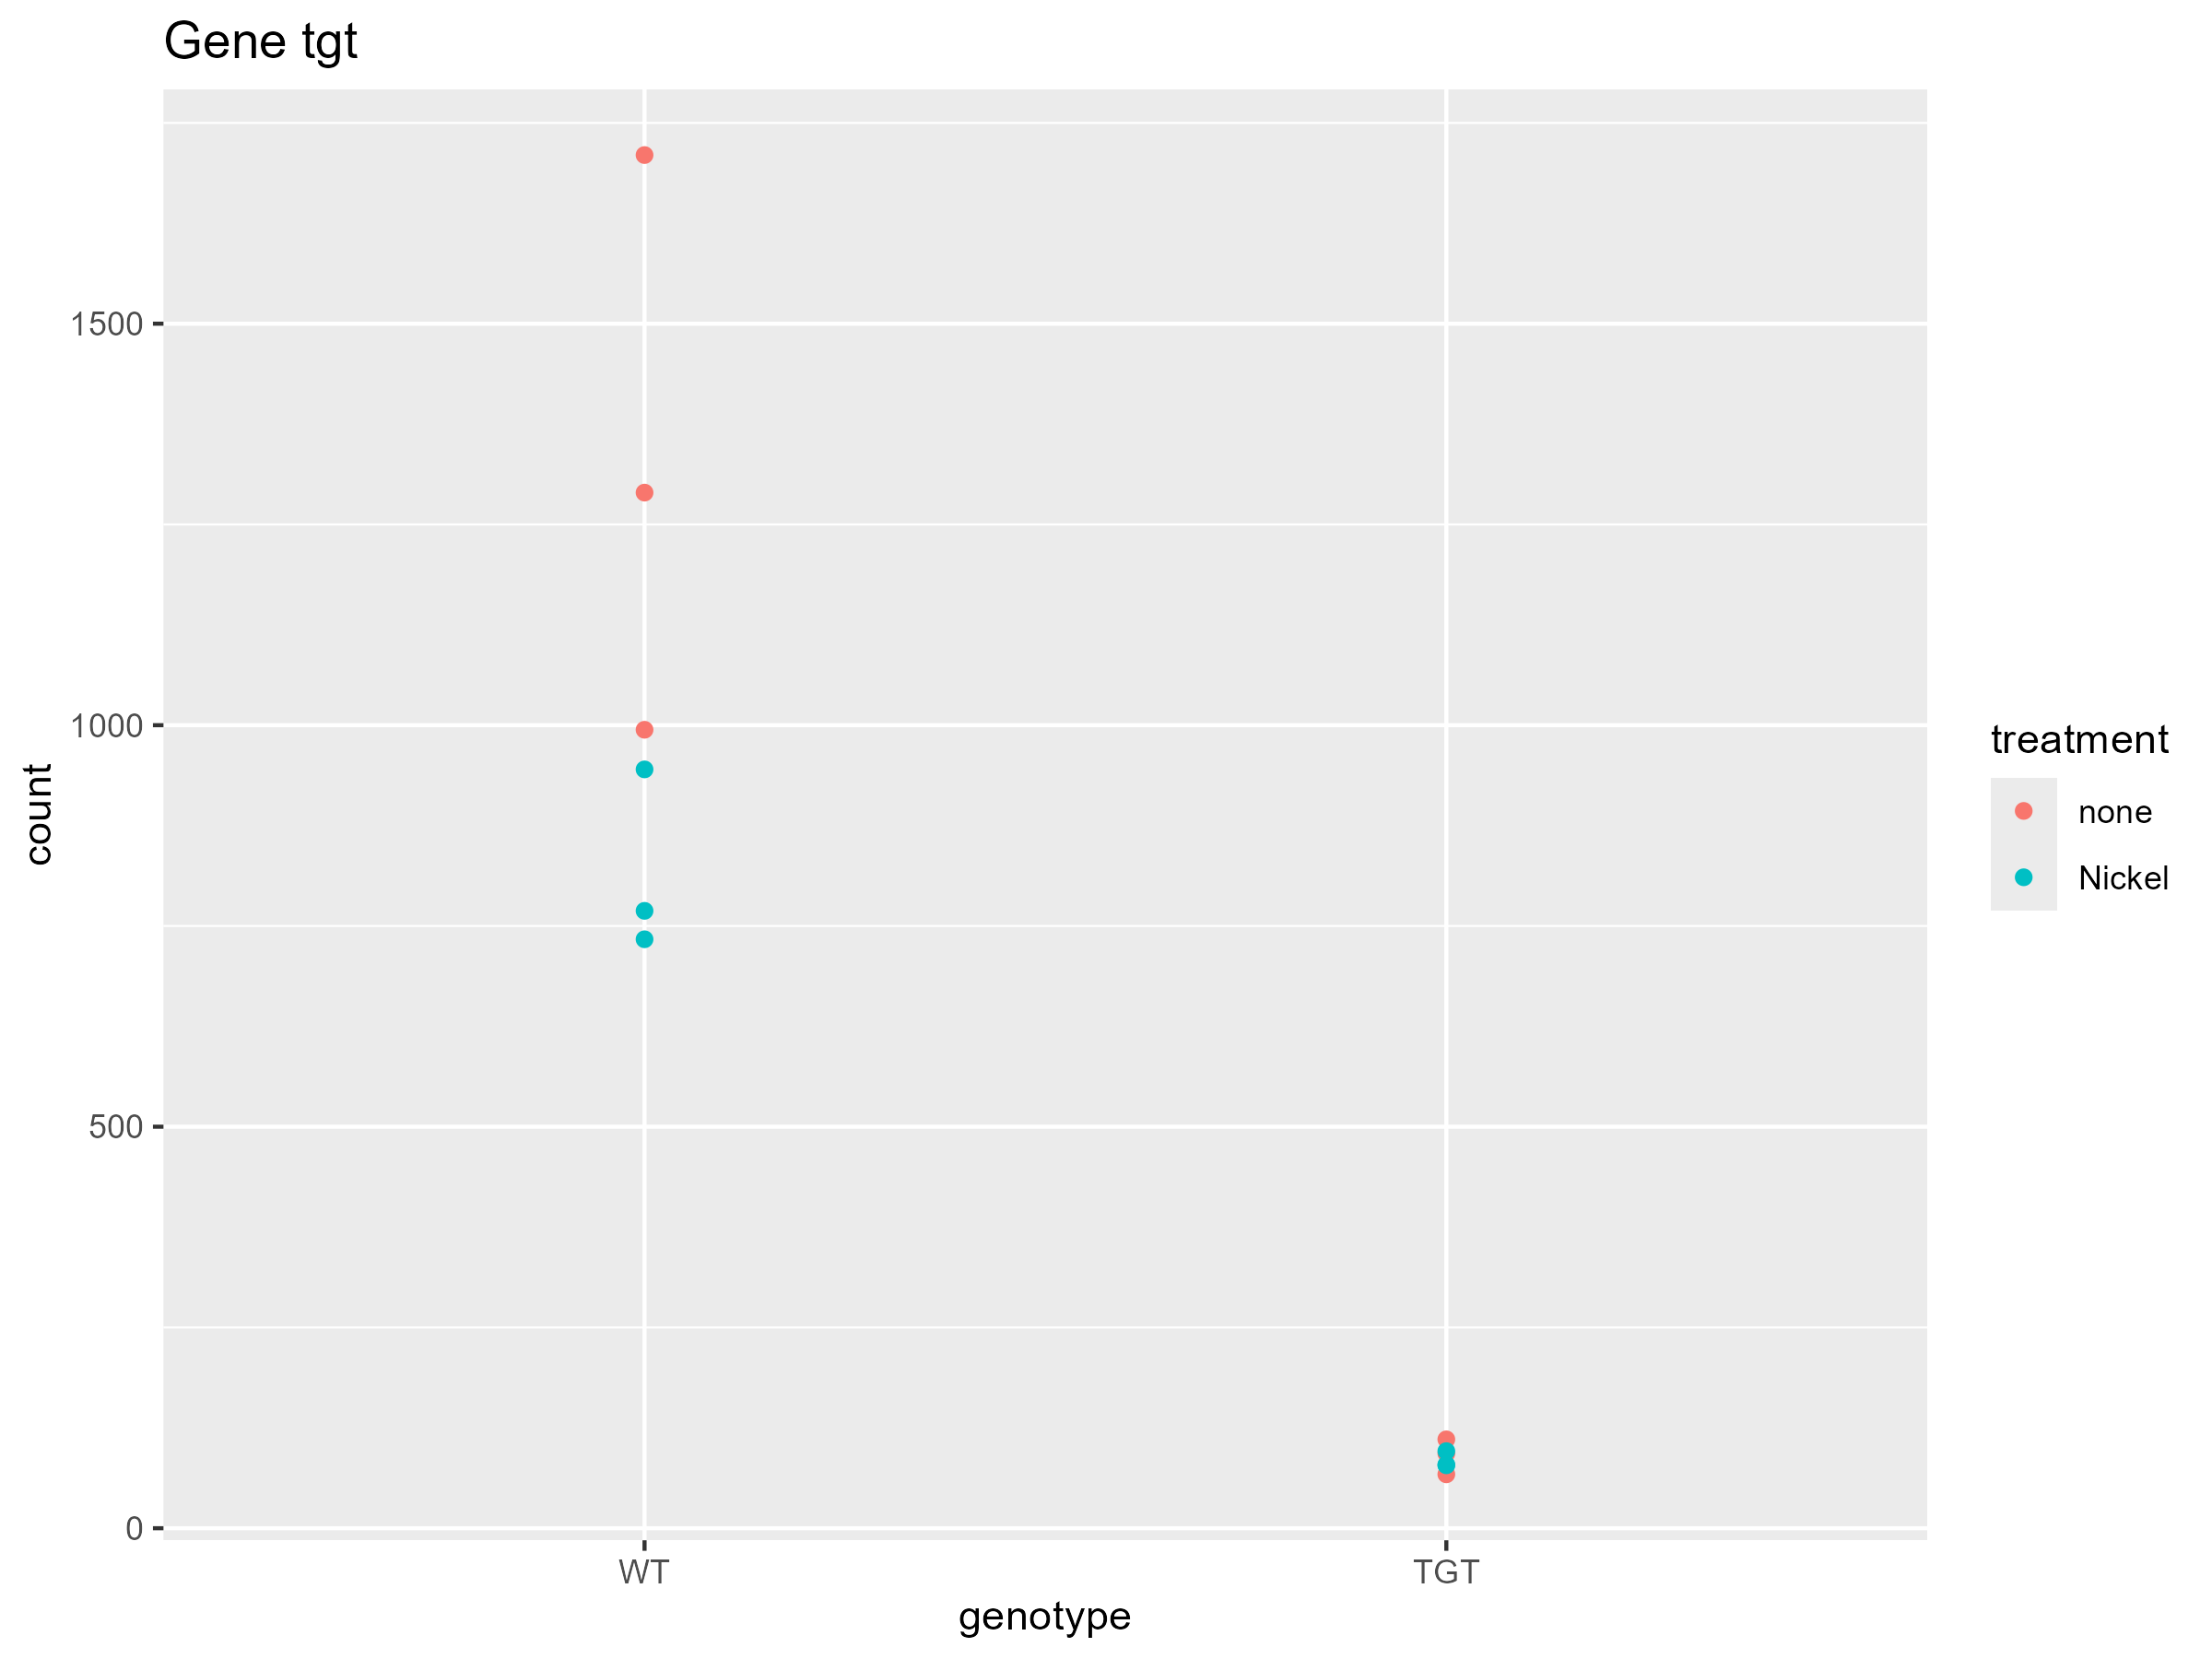
\includegraphics[width=0.85\linewidth]{TGTcounts} 

}

\caption{Expression counts for the tgt gene across all experimental conditions.}\label{fig:unnamed-chunk-11}
\end{figure}

\subsubsection{c) Expected tgt Gene Expression
Patterns}\label{c-expected-tgt-gene-expression-patterns}

The observed read count patterns for the tgt gene align with functional
expectations:

\textbf{WT + No Nickel:} Expected to show \textbf{high counts}. The tgt
gene encodes tRNA guanine transglycosylase, an essential enzyme for
queuosine synthesis, and is constitutively expressed during normal
growth.

\textbf{WT + Nickel:} Expected to show \textbf{lower counts than WT + No
Nickel}. Nickel stress causes transcriptional repression of the tgt
gene, resulting in reduced expression relative to untreated conditions.

\textbf{TGT Mutant + No Nickel:} Expected to show \textbf{very low to
near-zero counts}. The tgt gene is deleted in this strain, preventing
any functional transcript production.

\textbf{TGT Mutant + Nickel:} Expected to show \textbf{very low to
near-zero counts, similar to TGT + No Nickel}. The nickel-induced
repression is irrelevant in a deletion mutant, as no transcript is
produced regardless of treatment.

\newpage

\section*{References}\label{references}
\addcontentsline{toc}{section}{References}

\phantomsection\label{refs}
\begin{CSLReferences}{1}{0}
\bibitem[\citeproctext]{ref-R-rmarkdown}
Allaire, JJ, Yihui Xie, Christophe Dervieux, Jonathan McPherson, Javier
Luraschi, Kevin Ushey, Aron Atkins, et al. 2025. \emph{Rmarkdown:
Dynamic Documents for r}. \url{https://github.com/rstudio/rmarkdown}.

\bibitem[\citeproctext]{ref-DESeq22014}
Love, Michael I., Wolfgang Huber, and Simon Anders. 2014. {``Moderated
Estimation of Fold Change and Dispersion for RNA-Seq Data with
DESeq2.''} \emph{Genome Biology} 15: 550.
\url{https://doi.org/10.1186/s13059-014-0550-8}.

\bibitem[\citeproctext]{ref-R-DESeq2}
Love, Michael, Simon Anders, and Wolfgang Huber. 2025. \emph{DESeq2:
Differential Gene Expression Analysis Based on the Negative Binomial
Distribution}. \url{https://doi.org/10.18129/B9.bioc.DESeq2}.

\bibitem[\citeproctext]{ref-ggplot22016}
Wickham, Hadley. 2016. \emph{Ggplot2: Elegant Graphics for Data
Analysis}. Springer-Verlag New York.
\url{https://ggplot2.tidyverse.org}.

\bibitem[\citeproctext]{ref-R-tidyverse}
---------. 2023. \emph{Tidyverse: Easily Install and Load the
Tidyverse}. \url{https://tidyverse.tidyverse.org}.

\bibitem[\citeproctext]{ref-tidyverse2019}
Wickham, Hadley, Mara Averick, Jennifer Bryan, Winston Chang, Lucy
D'Agostino McGowan, Romain François, Garrett Grolemund, et al. 2019.
{``Welcome to the {tidyverse}.''} \emph{Journal of Open Source Software}
4 (43): 1686. \url{https://doi.org/10.21105/joss.01686}.

\bibitem[\citeproctext]{ref-R-ggplot2}
Wickham, Hadley, Winston Chang, Lionel Henry, Thomas Lin Pedersen,
Kohske Takahashi, Claus Wilke, Kara Woo, Hiroaki Yutani, Dewey
Dunnington, and Teun van den Brand. 2025. \emph{Ggplot2: Create Elegant
Data Visualisations Using the Grammar of Graphics}.
\url{https://ggplot2.tidyverse.org}.

\bibitem[\citeproctext]{ref-knitr2014}
Xie, Yihui. 2014. {``Knitr: A Comprehensive Tool for Reproducible
Research in {R}.''} In \emph{Implementing Reproducible Computational
Research}, edited by Victoria Stodden, Friedrich Leisch, and Roger D.
Peng. Chapman; Hall/CRC.

\bibitem[\citeproctext]{ref-knitr2015}
---------. 2015. \emph{Dynamic Documents with {R} and Knitr}. 2nd ed.
Boca Raton, Florida: Chapman; Hall/CRC. \url{https://yihui.org/knitr/}.

\bibitem[\citeproctext]{ref-R-knitr}
---------. 2025. \emph{Knitr: A General-Purpose Package for Dynamic
Report Generation in r}. \url{https://yihui.org/knitr/}.

\bibitem[\citeproctext]{ref-rmarkdown2018}
Xie, Yihui, J. J. Allaire, and Garrett Grolemund. 2018. \emph{R
Markdown: The Definitive Guide}. Boca Raton, Florida: Chapman; Hall/CRC.
\url{https://bookdown.org/yihui/rmarkdown}.

\bibitem[\citeproctext]{ref-rmarkdown2020}
Xie, Yihui, Christophe Dervieux, and Emily Riederer. 2020. \emph{R
Markdown Cookbook}. Boca Raton, Florida: Chapman; Hall/CRC.
\url{https://bookdown.org/yihui/rmarkdown-cookbook}.

\end{CSLReferences}

\end{document}
